\chapter{Конструкторская часть}

В данном разделе будут представлены схемы реализаций алгоритма полного перебора и муравьиного алгоритма для решения задачи коммивояжёра.

\section{Разработка алгоритма полного перебора для решения задачи коммивояжёра}
На рисунке \ref{img:bf} представлена схема реализации алгоритма полного перебора для решения задачи коммивояжёра. 

\begin{figure}[h!]
    \centering
    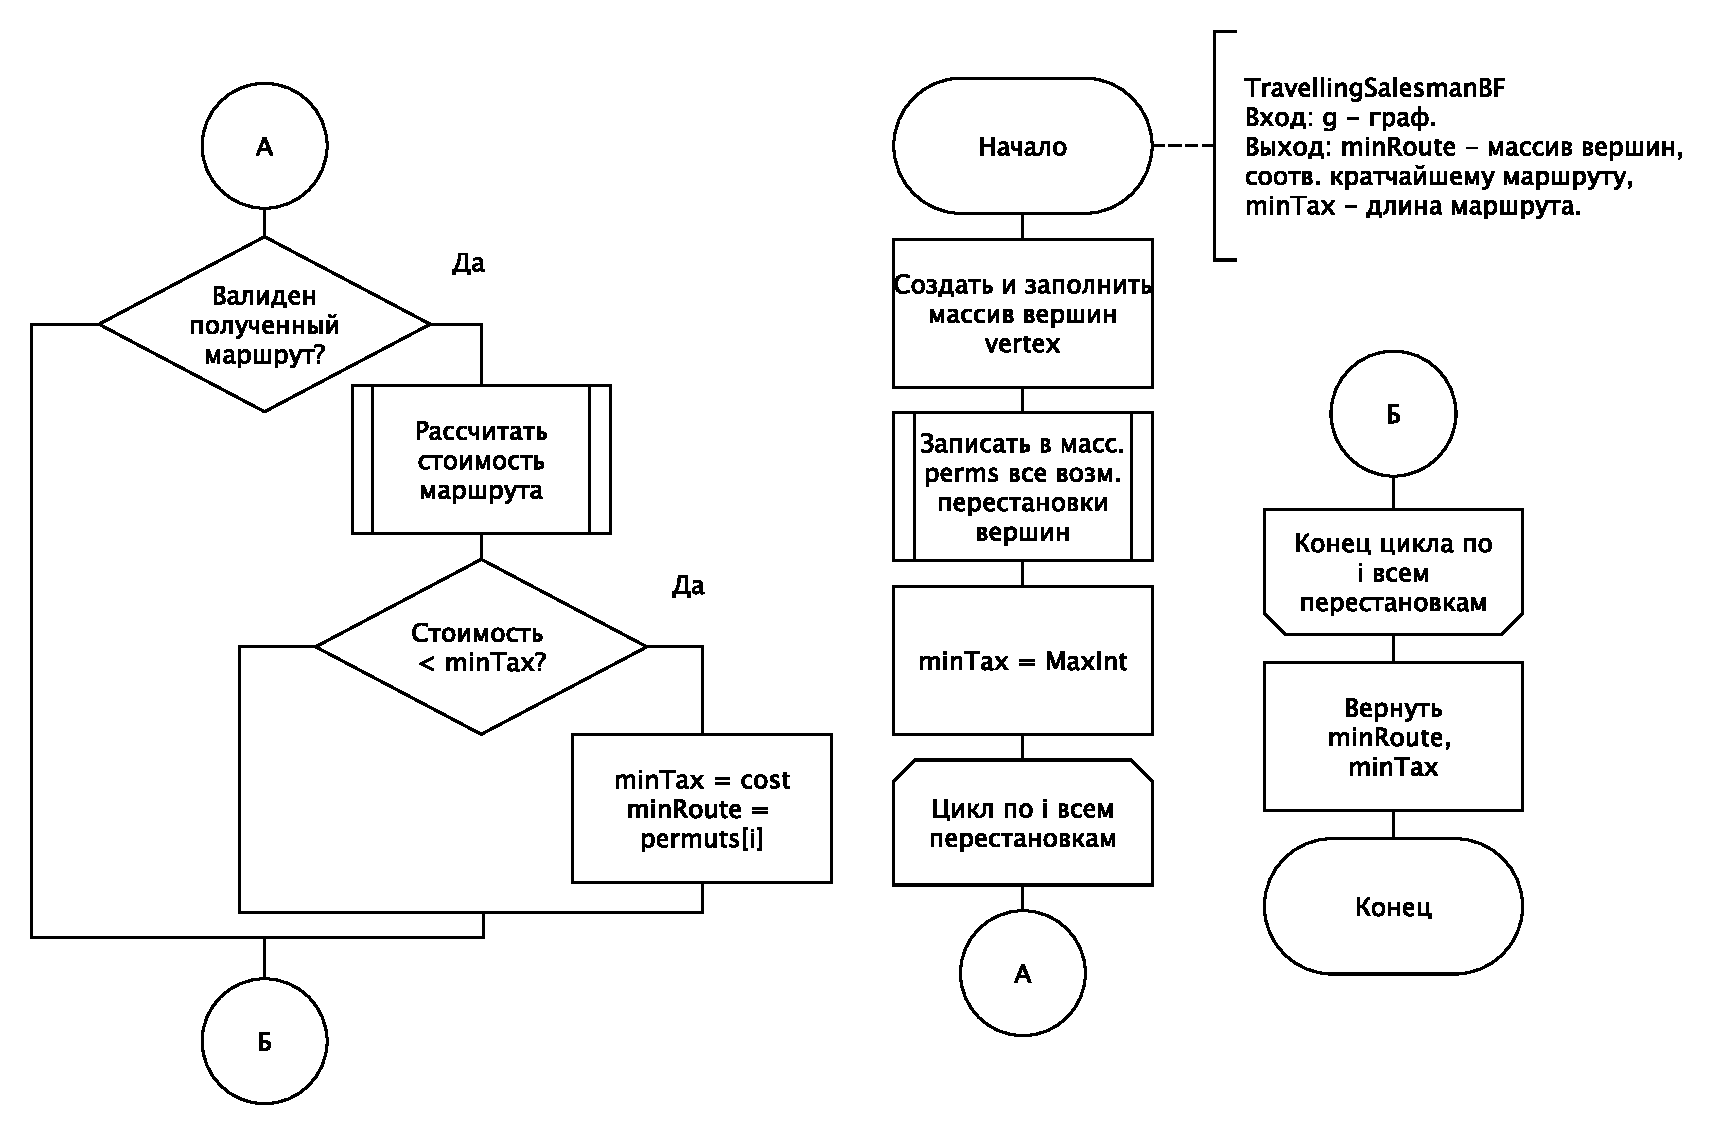
\includegraphics[width=0.95\linewidth]{bf.pdf}
    \caption{Схема реализации алгоритма полного перебора для решения задачи коммивояжёра}
    \label{img:bf}
\end{figure}

\section{Разработка муравьиного алгоритма для решения задачи коммивояжёра}
На рисунке \ref{img:aco} представлена схема реализации муравьиного алгоритма для решения задачи коммивояжёра, а на рисунках \ref{img:route}~--~\ref{img:go}~---~схемы необходимых для его реализации подпрограмм: поиска муравьём маршрута и поиска муравьём следующей вершины соответственно.

\begin{figure}[h!]
    \centering
    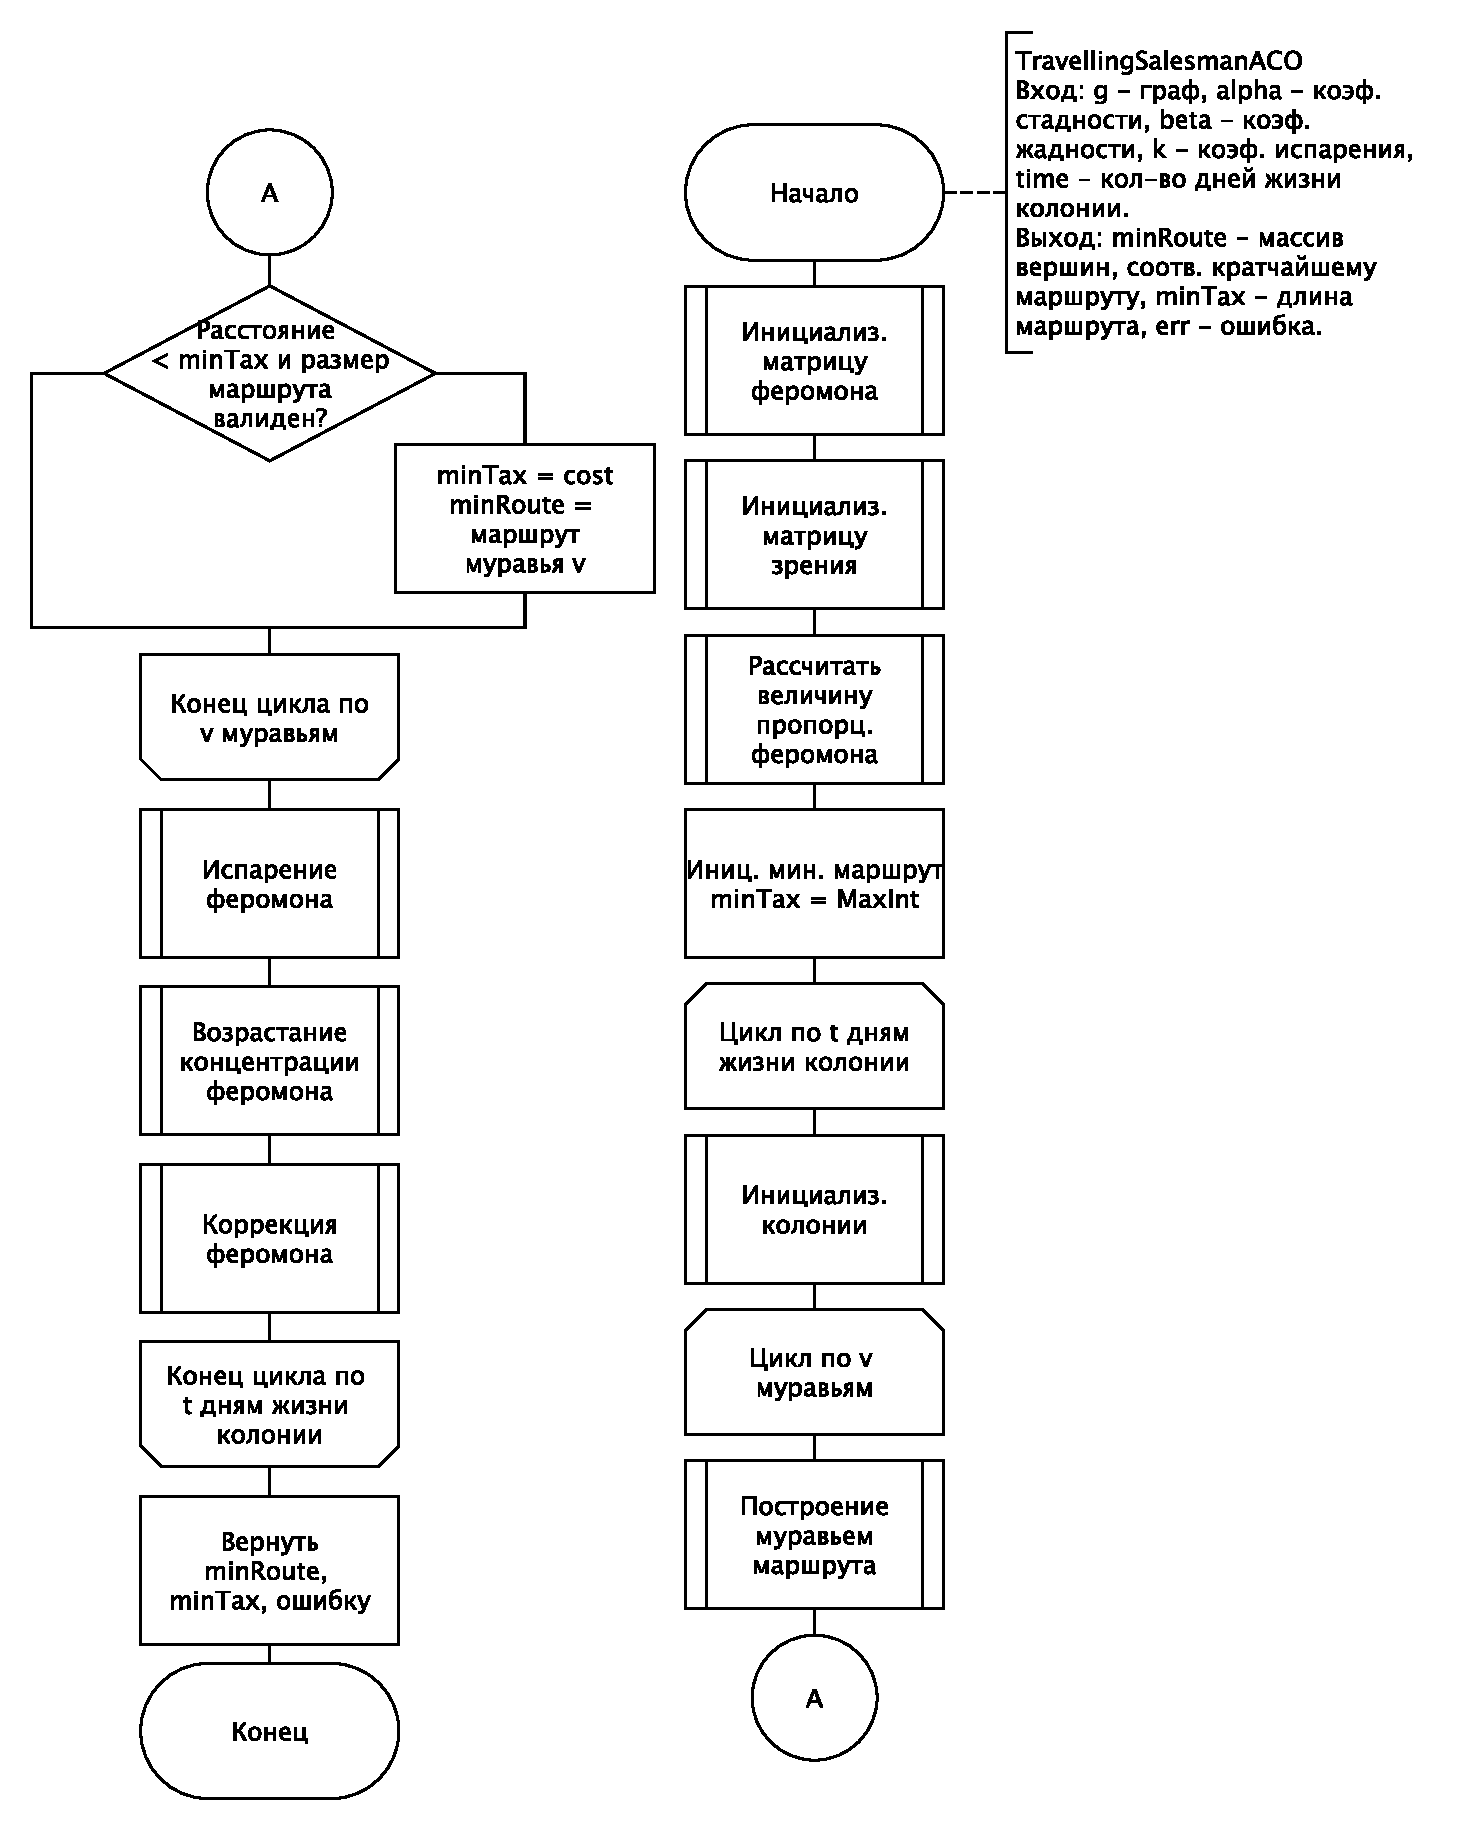
\includegraphics[width=0.7\linewidth]{aco.pdf}
    \caption{Схема реализации муравьиного алгоритма для решения задачи коммивояжёра}
    \label{img:aco}
\end{figure}

\newpage

\begin{figure}[h!]
    \centering
    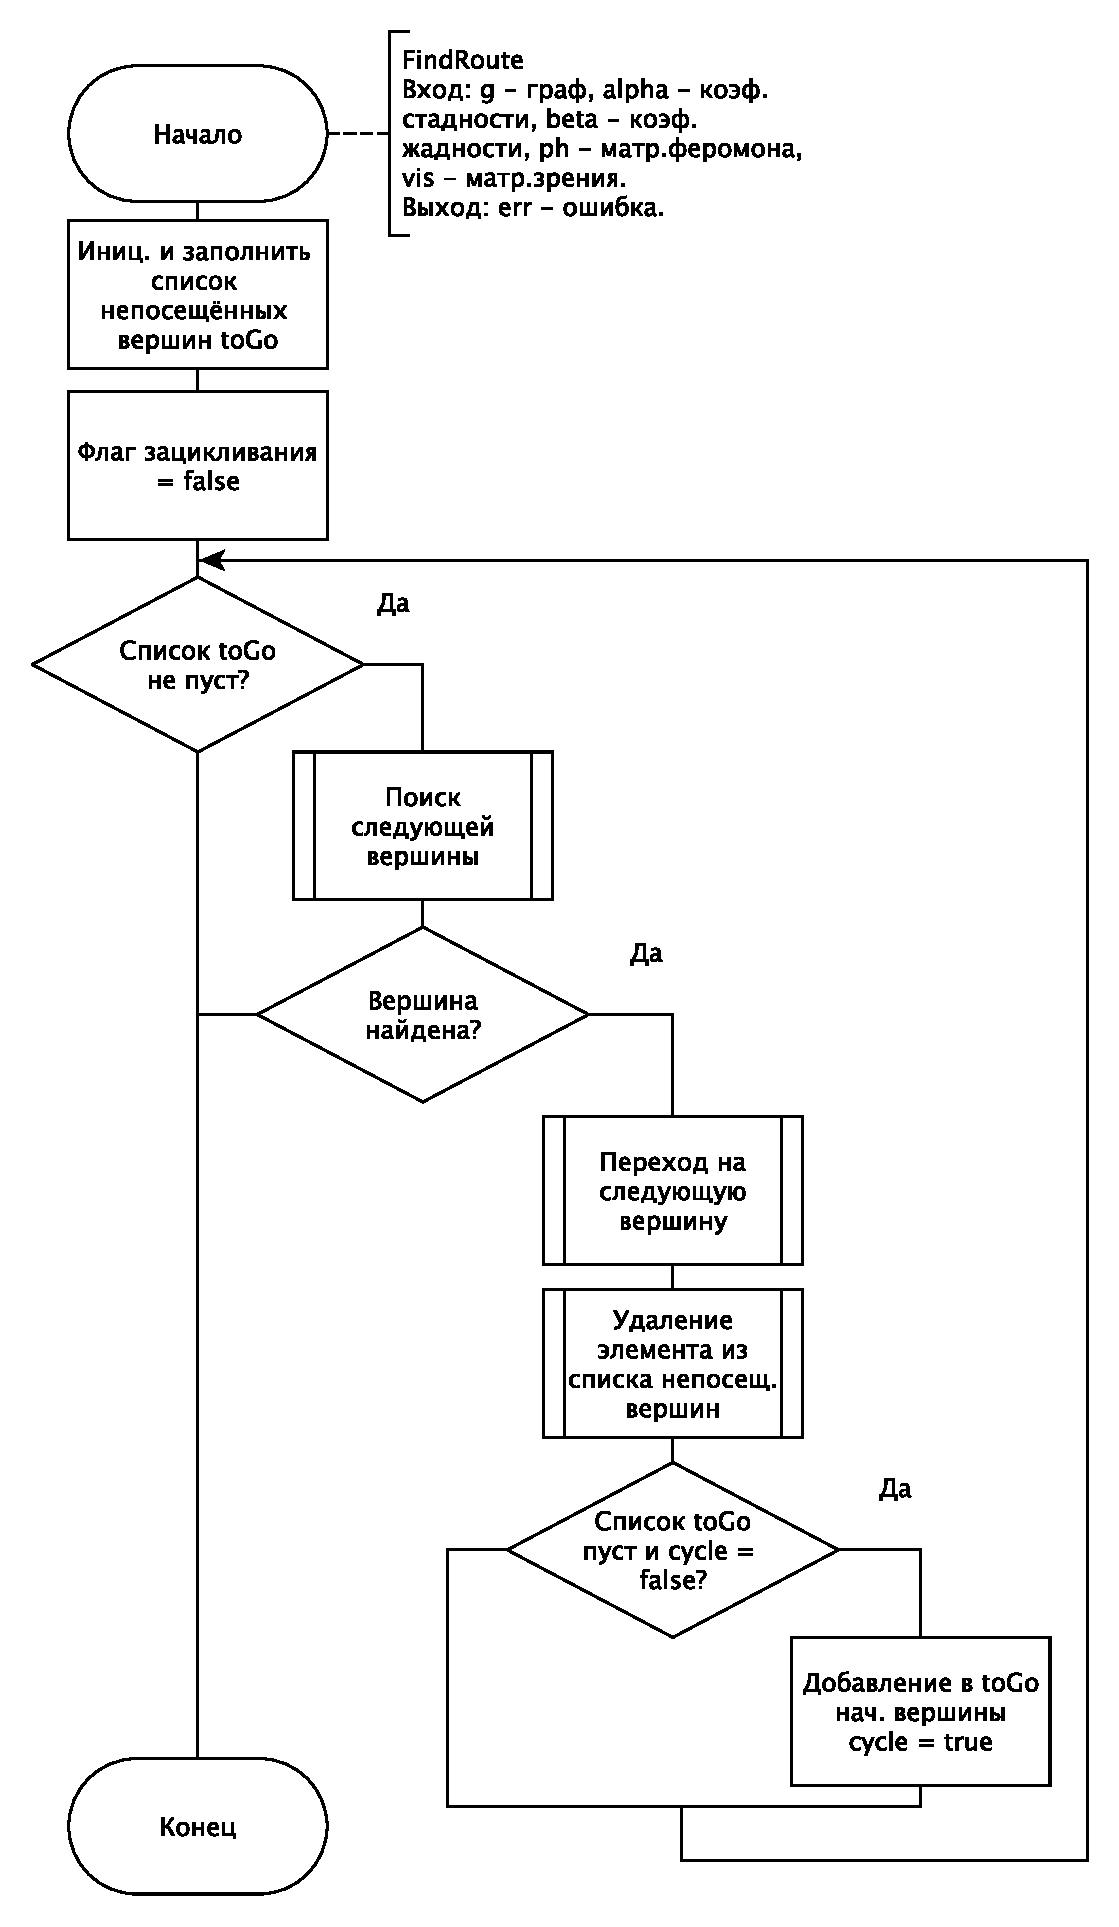
\includegraphics[width=0.7\linewidth]{route.pdf}
    \caption{Схема реализации алгоритма поиска муравьём маршрута}
    \label{img:route}
\end{figure}

\newpage

\begin{figure}[h!]
    \centering
    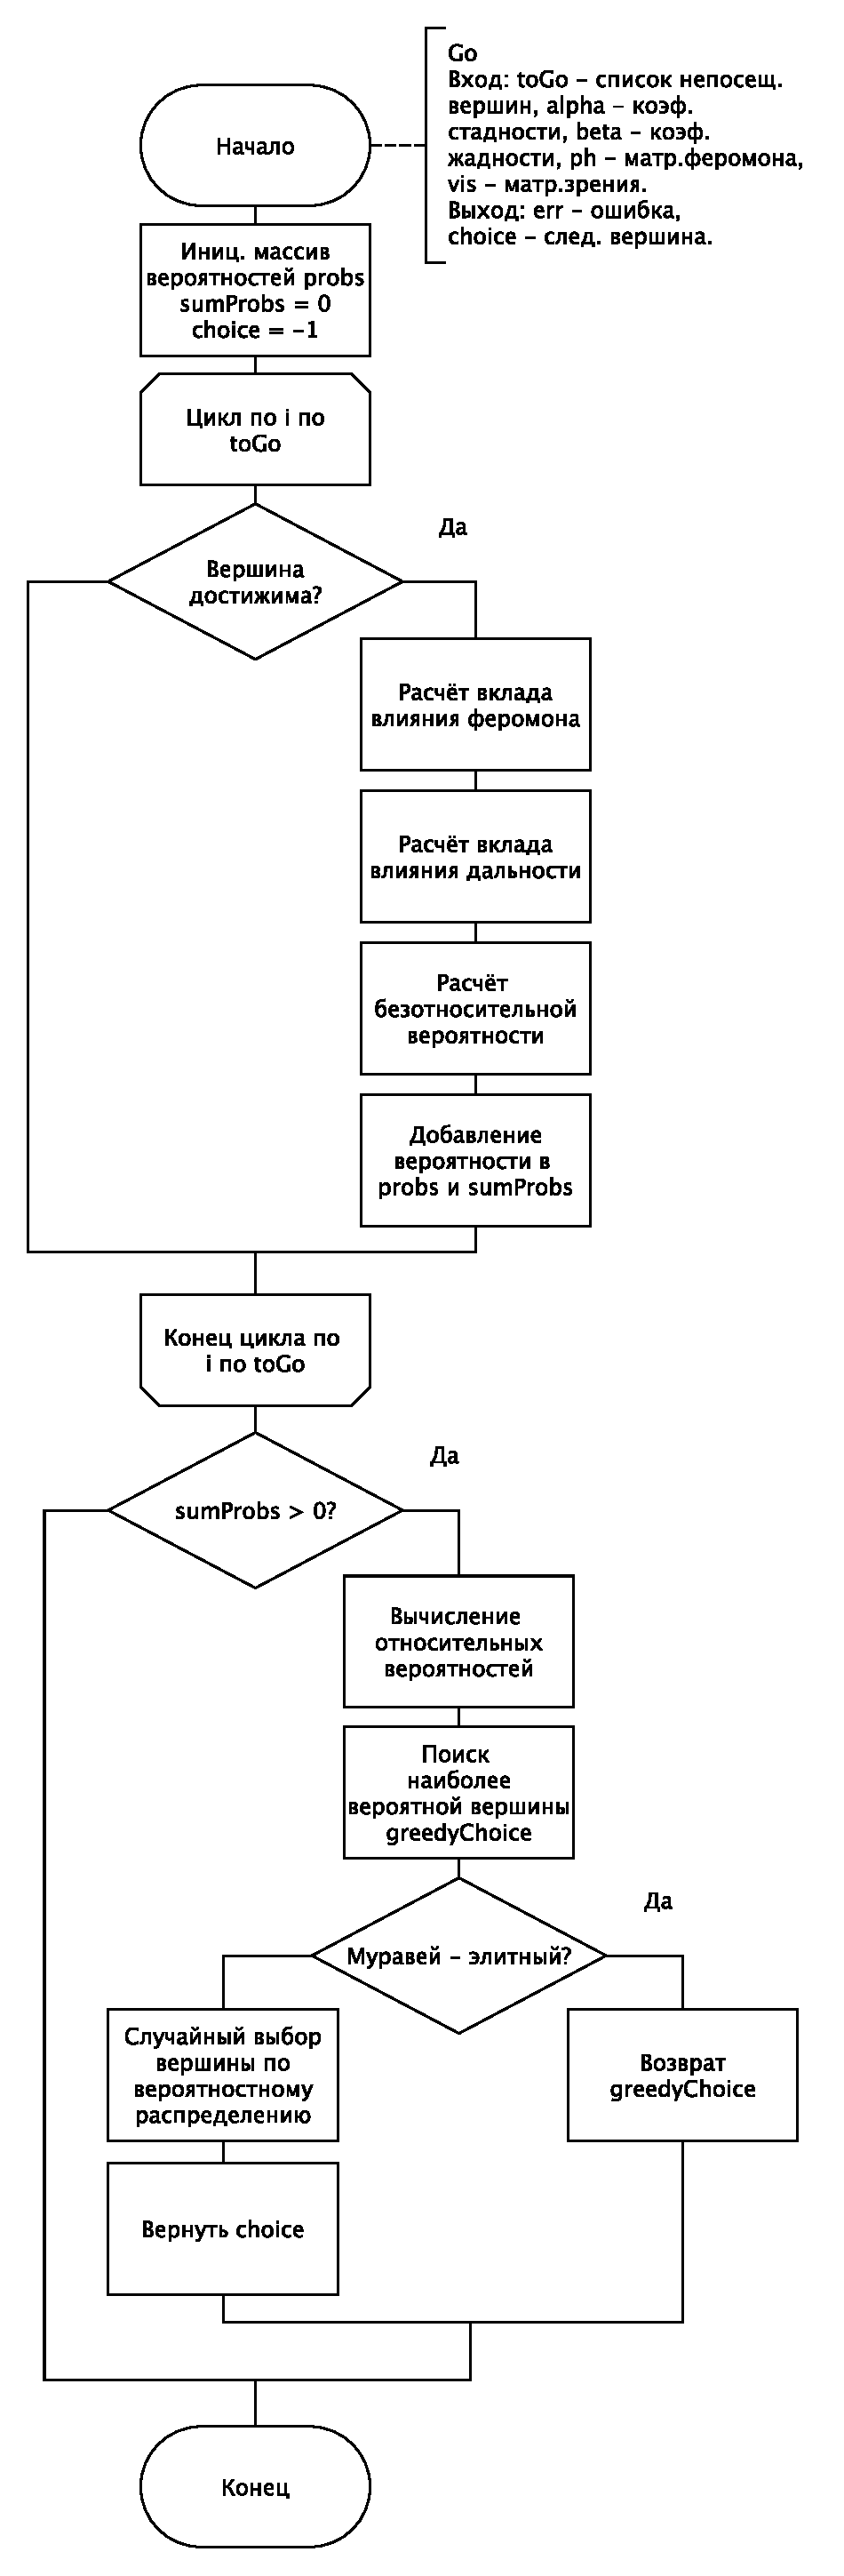
\includegraphics[width=0.4\linewidth]{go.pdf}
    \caption{Схема реализации алгоритма поиска муравьём следующей вершины}
    \label{img:go}
\end{figure}

\newpage

\section{Модель вычислений}
Для вычисления трудоёмкости данных алгоритмов необходимо ввести модель вычислений.

Обозначим трудоёмкость как $f_{a}$, где $a$~---~индекс, указывающий операцию, блок кода или оператор, для которого вычисляется трудоёмкость.

Определим трудоёмкость базовых операций как:
\begin{equation}
\begin{array}{rrrr}
	f_{+}=1 & \quad f_{-}=1 & \quad f_{+=}=1 & \quad f_{-=}=1 \\
	f_{:=}=1 & \quad f_{<<}=1 & \quad f_{>>}=1 & \quad f_{[]}=1 \\
	f_{++}=1 & \quad f_{--}=1 & \quad f_{>}=1 & \quad f_{<}=1 \\
	f_{>=}=1 & \quad f_{<=}=1 & \quad f_{!=}=1 & \quad f_{==}=1 \\
	f_{\cdot}=2 & \quad f_{/}=2 & \quad f_{\%}=2 & \quad \\
\end{array}
\end{equation}

Определим трудоёмкость вызова функции как $0$.

Определим трудоёмкость условия как

\begin{equation}
	f_{if} = f_{cc} + \begin{cases}
		\min(f_1, f_2),& \text{в лучшем случае}, \\
		\max(f_1, f_2),& \text{в худшем случае},
	\end{cases}
\end{equation}
где приняты следующие обозначения:
\begin{itemize}
	\item $f_{cc}$~---~трудоёмкость вычисления условия;
	\item $f_1$~---~трудоёмкость блока после $if$;
	\item $f_2$~---~трудоёмкость блока после $else$.
\end{itemize}

Определим трудоёмкость цикла как
\begin{equation}
	f_{loop} = f_{init} + f_{first-cmp} + n \cdot (f_{body} + f_{inc} + f_{cmp}),
\end{equation}
где приняты следующие обозначения:
\begin{itemize}
	\item $f_{init}$~---~трудоёмкость инициализации;
	\item $f_{first-cmp}$~---~трудоёмкость первого сравнения;
	\item $f_{body}$~---~трудоёмкость тела цикла;
	\item $n$~---~количество итераций цикла;
	\item $f_{inc}$~---~трудоёмкость изменения индекса;
	\item $f_{cmp}$~---~трудоёмкость сравнения.
\end{itemize}

\subsection{Трудоёмкость алгоритма полного перебора}

Трудоемкость алгоритма полного перебора решения задачи коммивояжера состоит из следующих составляющих.

Трудоёмкость внешнего цикла по $i \in [0..N!-1]$:
\begin{equation}
	f_{loop}= 2 + N! \cdot (2 + f_{body})
\end{equation}

Далее рассмотрена трудоёмкость для тела цикла в зависимости от результата проверки условия на существование заданного пути в графе:
\begin{equation}
  f_{body} = f_{if} + \begin{cases}
    f_{true}, & \text{если путь существует,}\\
    0, & \text{иначе.}
  \end{cases}
\end{equation}

Трудоёмкость проверки условия:
\begin{equation}
  f_{if} = 2 + N \cdot(2 + 8).
\end{equation}

Трудоёмкость действий при выполнении условия:
\begin{equation}
  f_{true} = 1 + 2 + N\cdot(2 + 10).
\end{equation}

Тогда трудоемкость алгоритма полного перебора решения задачи коммивояжера для лучшего случая (путь в графе не существует) составит
\begin{equation}
  f_{brute\_force} = 2 + N!\cdot(2 + 2 + N\cdot(2 + 8) ) = 2 + 4N! + 10N \cdot N! = O(N!),
\end{equation}
а трудоемкость для худшего случая (путь в графе существует):
\begin{equation}
\begin{aligned}
  f_{brute\_force} = 2 + N!\cdot(2 + 2 + N\cdot(2 + 8)  + 1 + 2 + N \cdot(2 + 10)) = \\ =2 + 7N! + 22N \cdot N! = O(N!).
\end{aligned}
\end{equation}

\section{Трудоёмкость муравьиного алгоритма}
Введём некоторые обозначения: $N$~---~размер графа (равен размеру муравьиной колонии), $T$~---~количество дней жизни колонии.

Далее приведён расчёт трудоёмкости муравьиного алгоритма для решения задачи коммивояжёра. 

Трудоёмкость внешней функции для муравьиного алгоритма:
\begin{equation} \label{eqn:4}
	f_{outer} = f_{ph} + f_{vis} + f_{q} + 2 + f_{loop-t} + 5.
\end{equation}

Трудоёмкость функции инициализации матрицы феромона:
\begin{equation}\label{eqn:5}
	f_{ph} = 1 + 2 + N \cdot (2 + 3) + 2 + N \cdot (2 + 2 + N \cdot(2 + 3)) = 5 + 7 \cdot N + 5 \cdot N^2.
\end{equation}

Трудоёмкость функции инициализации матрицы видимости:
\begin{equation}\label{eqn:6}
	f_{vis} = 1 + 2 + N \cdot (2 + 3) + 2 + N \cdot (2 + 2 + N \cdot(2 + 3)) = 5 + 7 \cdot N + 5 \cdot N^2.
\end{equation}

Трудоёмкость функции инициализации коэффициента пропорциональности феромона:
\begin{equation}\label{eqn:7}
	f_{q} = 1 + 2 + N \cdot (2 + 2 + N \cdot (2 + 3)) + 1 = 4 + 4 \cdot N + 5 \cdot N^2.
\end{equation}

Трудоёмкость цикла по дням:
\begin{equation}\label{eqn:8}
	f_{loop-t} = 2 + T \cdot (f_{col} + f{loop-n} + f_{vap} + f_{inc} + f_{cor}).
\end{equation}

Трудоёмкость функции создания колонии:
\begin{equation}\label{eqn:9}
	f_{col} = 1 + 2 + N \cdot (2 + 7) = 3 + 9 \cdot N.
\end{equation}

Трудоёмкость функции испарения феромона:
\begin{equation}\label{eqn:10}
	f_{vap} = 2 + N \cdot (2 + 2 + N \cdot (2 + 7)) = 2 + 4 \cdot N + 9 \cdot N^2.
\end{equation}

Трудоёмкость функции прироста феромона:
\begin{equation}\label{eqn:11}
	f_{inc} = 2 + N \cdot (2 + 2 + (N - 1) \cdot (2 + 9)) = 2 - 7 \cdot N + 11 \cdot N^2.
\end{equation}

Трудоёмкость функции коррекции феромона в лучшем случае (не нужна коррекцция) составит:
\begin{equation}\label{eqn:12}
	f_{cor} = 2 + N \cdot (2 + 2 + N \cdot 3) = 2 + 4 \cdot N + 3 \cdot N^2,
\end{equation}
а в худшем (нужна коррекция всех):
\begin{equation}\label{eqn:13}
	f_{cor} = 2 + N \cdot (2 + 2 + N \cdot 6) = 2 + 4 \cdot N + 6 \cdot N^2.
\end{equation}

Трудоёмкость цикла по количеству муравьёв в колонии:
\begin{equation}\label{eqn:14}
	f{loop-n} = 2 + N \cdot (2 + f_{route} + 8).
\end{equation}

Трудоёмкость функции поиска муравьём маршрута:
\begin{equation}\label{eqn:15}
\begin{aligned}
	f{route} = 1 + 2 + N \cdot (2 + 2) + 1 + f_{go}^{N - 1} + ... + f_{go}^{1} + f_{go}^{1} + N \cdot (5 + f_{rm} + 3) + 3 = \\ = 7 + 4 \cdot N + f_{go}^{N - 1} + ... + f_{go}^{1} + f_{go}^{1} + N \cdot (f_{rm} + 8).
\end{aligned}
\end{equation}

Трудоёмкость функции поиска муравьём следующей вершины для $n$ непосещённых вершин в лучшем случае (для 20\% элитных муравьёв):
\begin{equation} \label{eqn:16}
	f_{go} = 2 + 2 + (n - 1) \cdot (2 + 15) + 1 + 2 + 2 + (n - 1) \cdot (2 + 2 + 1) + 1 = -12 + 22 \cdot n,
\end{equation}
а в худшем (для обычных):
\begin{equation}\label{eqn:17}
	f_{go} = 2 + 2 + (n - 1) \cdot (2 + 15) + 1 + 2 + 2 + (n - 1) \cdot (2 + 2 + 4) + 2 + 3 + 2 + 4 \cdot n + 2 = -7 + 29 \cdot n.
\end{equation}

Трудоёмкость удаления элемента:
\begin{equation}\label{eqn:18}
	f_{rm} = 2 + N \cdot (2 + 9).
\end{equation}

Далее ведётся расчёт для лучшего случая.

Подставляется \ref{eqn:16} в \ref{eqn:15}:
\begin{equation} \label{eqn:19}
	f{route} = 7 + 4 \cdot N + (N-1) \cdot (-12) + (N-1) \cdot 22 \cdot \frac{N - 1 + 1}{2} + 10 + N \cdot (f_{rm} + 8).
\end{equation}

Подставляется \ref{eqn:18} в \ref{eqn:19}:
\begin{equation}
	f{route} = 7 + 4 \cdot N + (N-1) \cdot (-12) + (N-1) \cdot 22 \cdot \frac{N - 1 + 1}{2} + 10 + N \cdot (11 \cdot N + 10),
\end{equation}
что равняется 
\begin{equation}
	f{route} = 5 - 9 \cdot N + 22 \cdot N^2. 
\end{equation}

Для худшего случая аналогично получается
\begin{equation}
	f{route} = 7 + 4 \cdot N + (N-1) \cdot (-7) + (N-1) \cdot 29 \cdot \frac{N - 1 + 1}{2} + 10 + N \cdot (11 \cdot N + 10),
\end{equation}
что равняется 
\begin{equation}
	f{route} = 24 - 27.5 \cdot N + 25.5 \cdot N^2. 
\end{equation}

Подставив полученное в \ref{eqn:14} получим для лучшего случая:
\begin{equation}
	f{loop-n} = 2 + N \cdot (15 - 9 \cdot N + 22 \cdot N^2) = 2 + 15 \cdot N - 9 \cdot N^2 + 22 \cdot N^3,
\end{equation}
а для худшего:
\begin{equation}
	f{loop-n} = 2 + N \cdot (34 - 27.5 \cdot N + 25.5 \cdot N^2) = 2 + 34 \cdot N - 27.5 \cdot N^2 + 25.5 \cdot N^3.
\end{equation}

Далее выполним подстановку результатов в \ref{eqn:8} и приведём подобные слагаемые. Для лучшего случая:
\begin{equation}
	f_{loop-t} = 2 + 11 \cdot T + 25 \cdot N \cdot T + 14 \cdot N^2 \cdot T + 22 \cdot N^3 \cdot T,
\end{equation}
а для худшего:
\begin{equation}
	f_{loop-t} = 2 + 11 \cdot T + 44 \cdot N \cdot T - 1.5 \cdot N^2 \cdot T + 25.5 \cdot N^3 \cdot T.
\end{equation}

Подставив полученное в формулу \ref{eqn:4} для лучшего случая получается
\begin{equation}
	f_{outer} = 23 + 18 \cdot N + 15 \cdot N^2 + 11 \cdot T + 25 \cdot N \cdot T + 14 \cdot N^2 \cdot T + 22 \cdot N^3 \cdot T,
\end{equation}
а для худшего
\begin{equation}
	f_{outer} = 23 + 18 \cdot N + 15 \cdot N^2 + 11 \cdot T + 44 \cdot N \cdot T - 1.5 \cdot N^2 \cdot T + 25.5 \cdot N^3 \cdot T.
\end{equation}

Такую трудоёмкость можно оценить как $O(N^3 \cdot T)$.

\newpage